
\section{Introdução}


\noindent \begin{minipage}[c]{0.6\textwidth}
  \vspace {1cm}
  \par Esta presente aula prática tem por fim a aplicação dos paradigmas da linguagem orientada a objetos com a linguagem de programação Java\ref{fig:log_java}.
  \par Para os procedimentos práticos foi sugerido o uso de nome $gerenciaBanco$, o qual será implementado. A finalidade desta aula prática, visa a implementação de um sistema de gerenciamento de banco, aonde o cliente deste banco irá acendero sistema atravéz de uma interface gráfica através da biblioteca $java.swing.*$, o menu deverá ser do tipo $loop$ o usuário deverá escolher a oção de finalizar a operação.

\end{minipage}
\begin{minipage}[c]{0.4\textwidth}

  
\includegraphics[width=\textwidth]{figure/log_java.jpg}
  	\label{fig:log_java}
    \captionof{figure}{Logo Java, \cite{logJava}}
    %\captionof*{figure}{Fonte: \citeonline{linux:2023}}
\end{minipage}

\par As funções para este programa são:
\begin{itemize}
  \item Incerção das credenciais (Nome, Sobrenome e cpf);
  \item Consulta de saldo;
  \item Depósito;
  \item Saque;
  \item Finaliza a operação com uma mensagem de despedida;
\end{itemize}

\section{Métodos}
\par Para a organização desta aula prática foi conficcionado um diagrama UML para o programa, conforme demonstra a figura \ref{fig:uml}

\begin{figure}[h]
  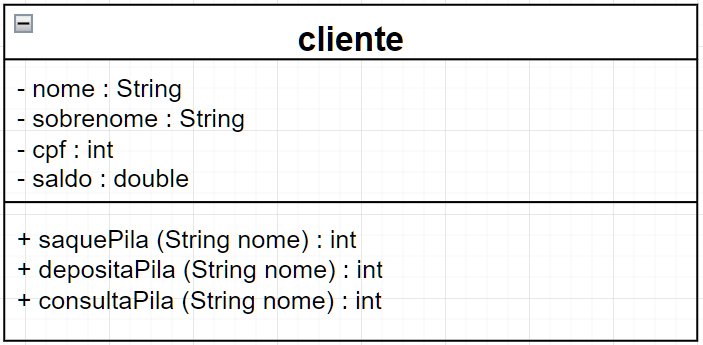
\includegraphics[width=\textwidth]{figure/uml_classe.png}
  \caption{Diagirama UML, O autor}
  \label{fig:uml}
\end{figure}
\newpage
\par Os atributos defenidos são:
\begin{itemize}
  \item name : String
  \item sobrenome : String
  \item cpf : String
  \item saldo : double
\end{itemize}

\par segundo boas práticas de programação, é sugerido que realize estencivamente controle de erros, e para tal, a criação de constatnte de verificação em vez de zeros e uns (0,1), do tipo $private static final int  STATUS\_OK = 1;$.

\section{Resultados}






\subsection{Métodos das classes}

\par Os métodos definem as ações da classe, eu acesso é $minhaClasse.meuMetodo(args)$

\begin{lstlisting}[language=Java, caption=consultaPilas, label=consultaPilas]
    /**
     * @param nome da conta a ser consultado
     * @return Retorna o saldo da conta
     */
     public double consultaPilas(String nome){

         return this.saldo;
     }

\end{lstlisting}

\begin{lstlisting}[language=Java, caption=depositoPilas, label=depositaPilas]
    /**
   * @param nome da conta a ser depositado
   * @return 1 se deu certo e 0 se ocorreu um erro
   */
   public void depositaPila(double pilas, String nome){

       this.saldo += pilas;
   }
\end{lstlisting}


%\lstinputlisting[language=Java]{GerenciaBanco.java} %Busca os codigos na pasta /cod






\begin{equation}
S = \left\{
\begin{aligned}
  a + b     &= 4\\
  a \cdot b &= 4
\end{aligned}
\right.
$$ $$% Usado para pular linha [não recomendado]
\sum_{n<k,\;\text{$n$ odd}} nE_n
 \label{1}
\end{equation}


\section{Conclusões}


\begin{enumerate}[label=\Roman{*}, ref=(\roman{*})]
  \item fsfsdf
  \item kugfhiuh
\end{enumerate}

\begin{asparaenum}
\item Anterior ... \cite{ninguem2022curioso}
\item Próximo ... \label{pl1}
\end{asparaenum}









  %$X \xLongleftarrow[\text{NATAN}]{\text{OGLIARI}} Y $ %COM TEXTO
	% $\uparrow$ %Seta para Cima
	%$\overleftarrow{NATAN}$
